\subsection{OpenCL}
The project requires interaction with heterogeneous processing devices present within a user's system.
It achieves this via the hardware vendor's implementation of the \ac{OpenCL} library.

\ac{OpenCL} is an open framework for executing tasks, described by C99-syntax \emph{kernels}, on a variety of devices.
Suitable targets include a range of heterogeneous devices such as multi-core \acp{CPU}, \acp{APU}, and \ac{GPU} from the majority of commodity hardware vendors.

The Khronos Group maintains and frequently updates the \ac{OpenCL} standard\cite{khronos}.
Participating vendors include \ac{AMD}, Apple, Intel, and NVIDIA \textemdash{} although the quality and accessibility of implementations varies greatly.

A stated goal of the \ac{OpenCL} project is to ``allow cross-platform parallel programming''.
The underlying processing devices present on a system are abstracted, allowing code to be written without explicit knowledge of target architectures.
This theoretically enables developers to write applications for a person system and then later scale execution to a massively parallel workstation, without significant code modification.

\begin{figure}[h]
	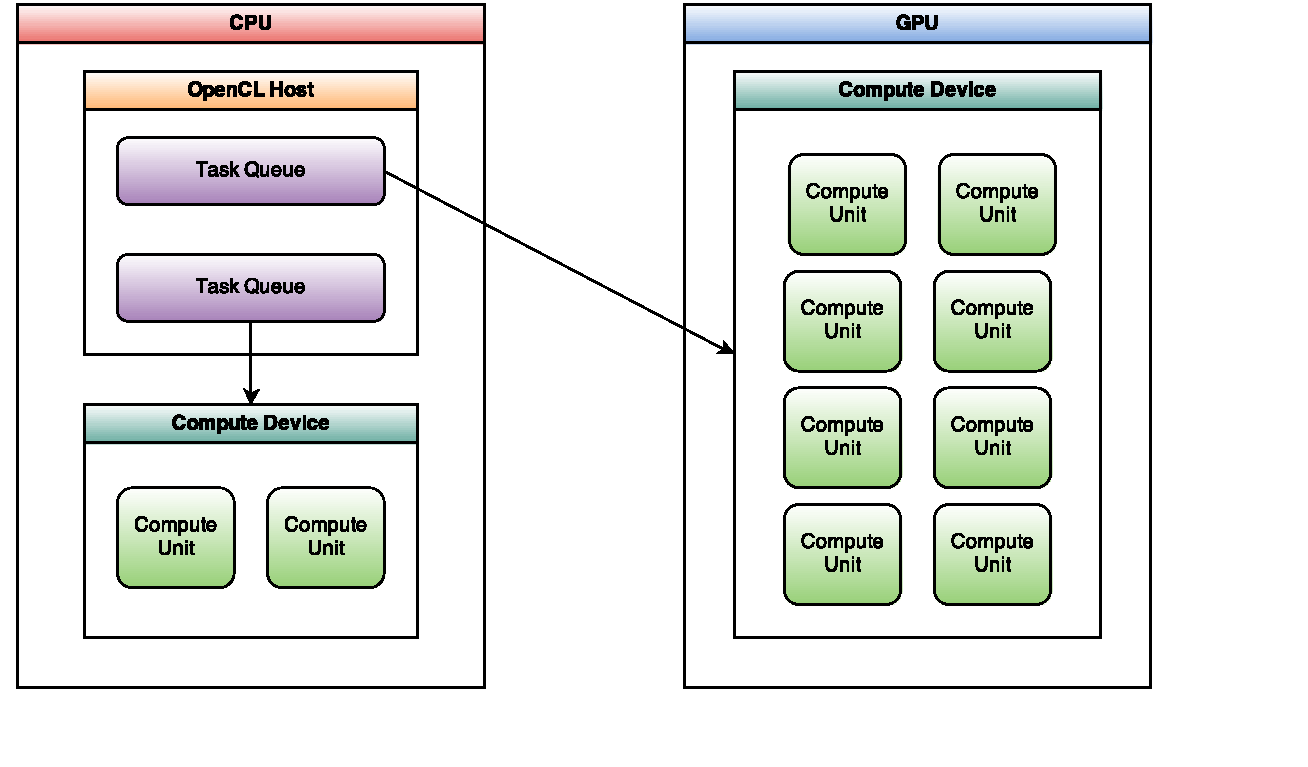
\includegraphics[width=3.8in]{./figures/OpenCLModel}
	\captionof{figure}{The OpenCL architecture model.}
	\label{fig:ocl_model}
\end{figure}

\paragraph{Architecture model}
As Figure~\ref{fig:ocl_model} illustrates, the architecture model presented by \ac{OpenCL} is as follows:

\begin{description}
\item[Host device] The system's \ac{CPU}. It interacts with an execution environment, responsible for discovering and selecting compute devices present on the system. The host device initialises one or more \emph{contexts}, whereby any devices within a single context have access to shared task and memory buffers.

\item[Compute devices] The system's available processing devices, capable of scheduling \ac{OpenCL} kernel work-groups. Before enumerating compute devices, the available \emph{platforms} must be discovered by the runtime. Usually, there is a platform presented for each unique \ac{OpenCL} supporting vendor with hardware installed. Devices are then retrieved on a per-platform bases, either filtered by type (\ac{CPU}/\ac{GPU}) or not.

\item[Compute Units] Discrete units of hardware present within a processing devices, capable of scheduling and executing \ac{OpenCL} kernel instances.
Kernel execution occurs across internal \emph{processing units}, such as \acp{ALU}.
\end{description}

\paragraph{Execution Model}
\ac{OpenCL} has a simple execution model, allowing both \emph{coarse-grained} and \emph{fine-grained} parallelism. Programmers write parallel code from the reference frame of a single kernel execution. Each instance orients itself only via access to its \emph{local} and \emph{global} \verb|id|, expanded on shortly. Larger calculations are a direct result of cooperating kernel instances. 

Kernel instances, scheduled for execution on compute devices, as referred to as \emph{work-items}.

The \ac{OpenCL} standard calls a collection of work-items a \emph{work-group}. Work-groups are the unit of work dispatched to a device. The number of work-items within a group that a device should schedule is set by the programmer, providing the \verb|global_work_size| parameter. Each kernel invocation is enumerated with a global \verb|id|. 

In addition to flat enumeration, the computation can benefit from the abstraction of work \emph{dimensions}. For example, a calculation over $100$ elements can represented as a 2-dimensional $10 \times 10$ calculation. When utilising dimensional abstraction, access to either unique global \verb|id| or $x, y$ offsets is available.

Higher dimensions are available for further structuring of tasks. It is clear that the spatial abstraction provided when there is a topological significant within the processed data. In these circumstances, the \verb|local_work_size| parameter provides further benefits.

When \verb|local_work_size| is specified, again possibly with dimensionality, the work-items are additionally divided into subgroups. Memory allocation can use the \verb|__local| qualifier. In this case, data will reside in higher-bandwidth buffers that can only be synchronised between members of the same local work-group. With the addition of this second, local tier of memory, the \ac{OpenCL} model hints at how efficient kernels should be constructed. Being aware of the positioning of data and its dependencies is key to developing efficient kernels, free of memory-synchronisation bottlenecks.

Much of the project's implementation effort concerning \ac{OpenCL} will be mapping data required by common algorithms to efficient arrangements within device memory. This mirrors \ac{OpenCL} development in general.
The fact that this task is so laborious is a reason why heterogeneous parallel programming is still under-utilised in the wild.


